\documentclass{article}
\usepackage{amsmath}
\usepackage{amssymb}
\usepackage{indentfirst}
\usepackage{graphicx}
\usepackage{color}
\usepackage{fancyhdr}
\usepackage{epstopdf}
\usepackage{indentfirst}
\usepackage{geometry}
\geometry{left=2.5cm,right=2.5cm,top=2.5cm,bottom=2.5cm}

\title{14.03 Problem Set 4}
\author{Yijun Jiang}
%\email{yjjiang@mit.edu}
\date{\today}

\pagestyle{fancy}
\lhead{Yijun Jiang}
\rhead{14.03 Problem Set 4}

\begin{document}
\maketitle

\section{International Trade}
\subsection{Part 1}
Since $X=L_X$ and $Y=5\sqrt{L_Y}$, we have $L_X=X$ and $L_y=Y^2/25$. Therefore, the Finnish PPF is
\begin{equation*}
X+\frac{1}{25}Y^2=300
\end{equation*}

This PPF is plotted in Fig.\ref{PPF}.
\begin{figure}[!htbp]
\centering
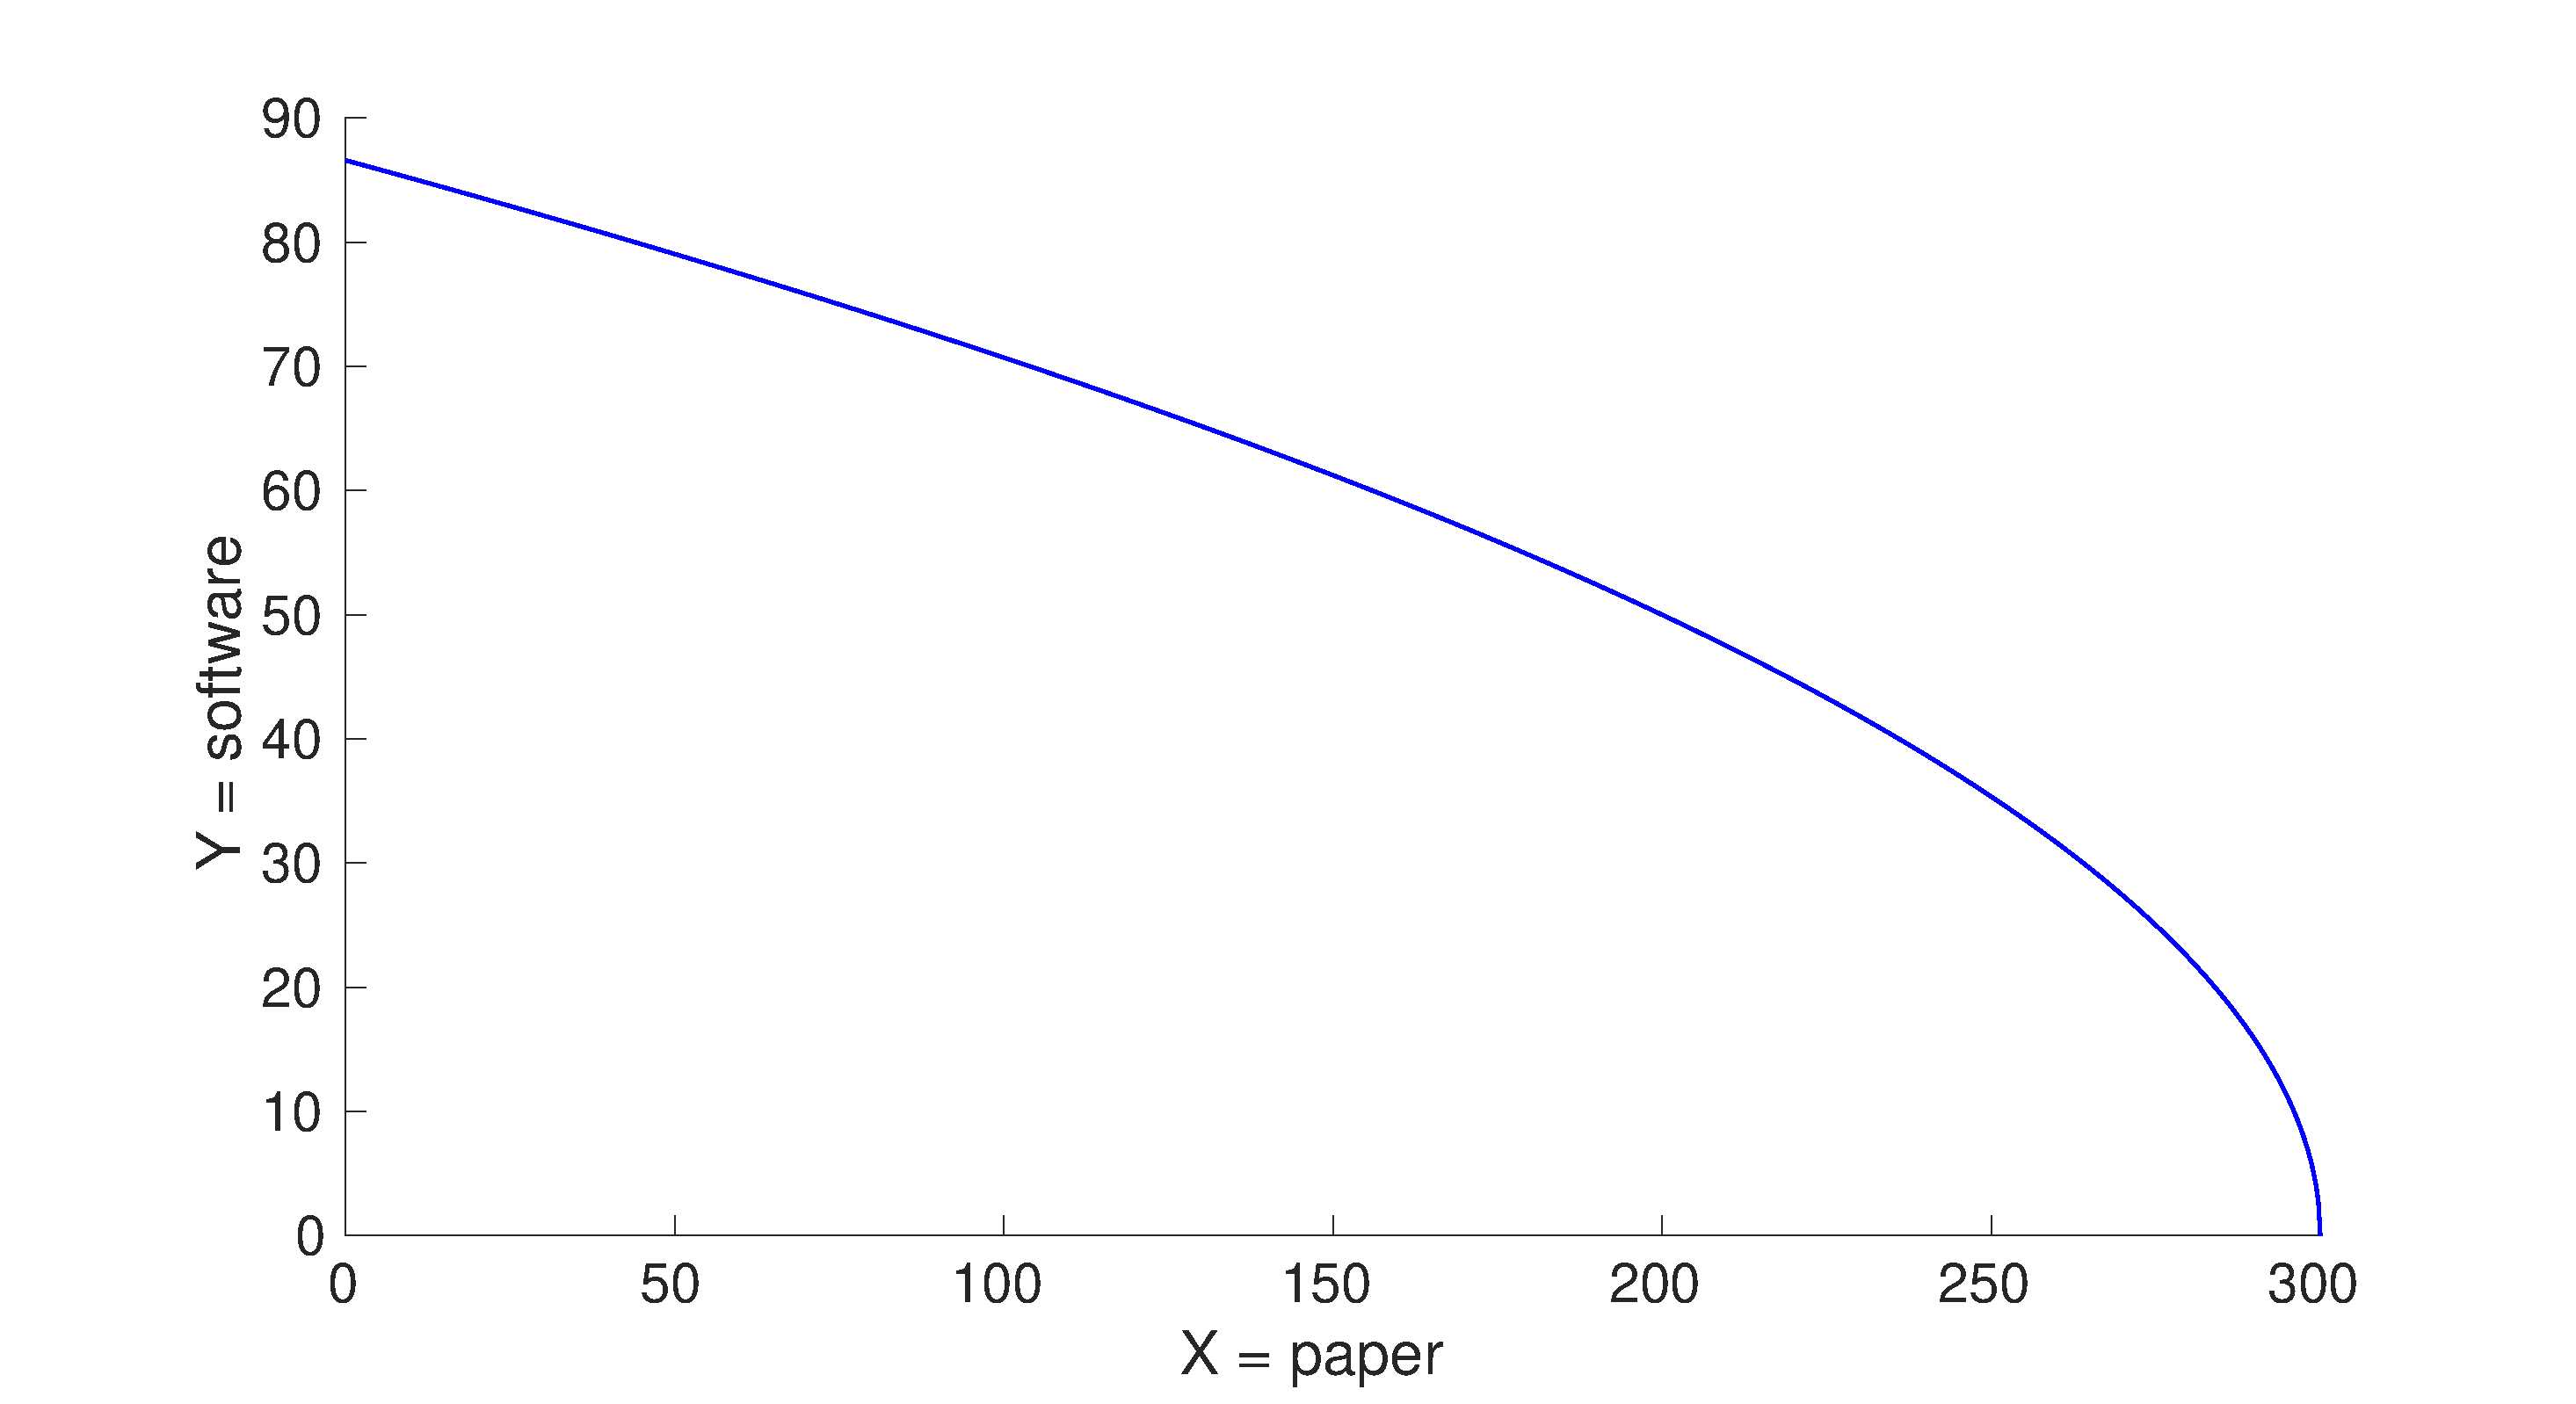
\includegraphics[width=12cm]{PPF.eps}\\
\caption{Finnish PPF for paper ($X$) and software ($Y$) production}\label{PPF}
\end{figure}

\subsection{Part 2}
MRS is given by
\begin{equation*}
\textup{MRS}_{XY}=\frac{\partial U/\partial X}{\partial U/\partial Y}=\frac{U/3X}{U/3Y}=\frac{Y}{X}
\end{equation*}

The PPF is
\begin{equation*}
\textup{PPF}(X,Y)=X+\frac{1}{25}Y^2-300=0
\end{equation*}

MRT is given by
\begin{equation*}
\textup{MRT}_{XY}=\frac{\partial\textup{PPF}/\partial X}{\partial\textup{PPF}/\partial Y}=\frac{1}{2Y/25}=\frac{25}{2Y}
\end{equation*}

\subsection{Part 3}
If Finland does not trade with other countries, its MRS must equal MRT. Also, the bundle must lie on the PPF curve.
\begin{align*}
&\frac{Y}{X}=\frac{25}{2Y}\\
&X+\frac{1}{25}Y^2=300
\end{align*}

The solution is
\begin{equation*}
(X^A,Y^A)=(200,50)
\end{equation*}
where the superscript $A$ stands for autarky. So Finland produces 200 units of paper ($X$) and 50 units of software ($Y$).

The equilibrium price ratio is
\begin{equation*}
\frac{P^F_Y}{P^F_X}=\textup{MRT}_{YX}=\frac{1}{\textup{MRT}_{XY}}=\frac{2Y^D}{25}=4
\end{equation*}

\subsection{Part 4}
Since $P^U_X=P^F_X=1$ and $P^U_Y>P^F_Y$, the US has comparative advantage over paper ($X$) and Finland has comparative advantage over software ($Y$). Therefore, if trade begins, Finland will export software and the US will export paper.

Since $P^U_X=P^F_X=1$, to result in no trade, the US software price must equal that of Finland: $P^U_Y=P^F_Y$.

\subsection{Part 5}
Let MRT equal the price ratio.
\begin{equation*}
MRT_{XY}=\frac{25}{2Y}=\frac{P_X^I}{P_Y^I}=\frac{1}{4.8}
\end{equation*}
which gives $Y^T=60$, where the superscript $T$ stands for trade. Consequently, $X^T=300-(Y^T)^2/25=156$. So Finland produces 156 units of paper ($X$) and 60 units of software ($Y$). The GDP is
\begin{equation*}
\textup{GDP}=P_X^IX^T+P_Y^IY^T=1\times 156+4.8\times 60=444
\end{equation*}

\subsection{Part 6}
We try to maximize $U(X,Y)=X^{1/3}y^{1/3}$ subject to the constraint that $P_X^IX+P_Y^IY\leqslant\textup{GDP}=444$. Introduce a Lagrange multiplier $\lambda$,
\begin{equation*}
L(X,Y,\lambda)=X^{1/3}Y^{1/3}-\lambda(X+4.8Y-444)
\end{equation*}

Taking partial derivatives with respect to $X,Y$ and $\lambda$ and setting them to zero,
\begin{align*}
&\frac{1}{3}X^{-2/3}Y^{1/3}=\lambda\\
&\frac{1}{3}X^{1/3}Y^{-2/3}=4.8\lambda\\
&X+4.8Y=444
\end{align*}

The solution is
\begin{equation*}
(X^*,Y^*)=(222,46.25)
\end{equation*}

Therefore, the excess demand of paper ($X$) is $\Delta X=X^*-X^T=222-156=66$, and the excess demand of software ($Y$) is $\Delta Y=Y^*-Y^T=46.25-60=-13.75$. This means Finland will import 66 units of paper and export 13.75 units of software.

In the autarky case, Finnish utility is
\begin{equation*}
U^A=(X^A)^{1/3}(Y^A)^{1/3}=(200\times 50)^{1/3}\approx21.54
\end{equation*}

In the trading case, Finnish utility is
\begin{equation*}
U^T=(X^*)^{1/3}(Y^*)^{1/3}=(222\times 46.25)^{1/3}\approx21.73
\end{equation*}

Since $U^T>U^A$, a representative Finnish consumer is better off when Finland opens to trade.

\subsection{Part 7}
Since Finland produces more software and less paper when it opens to trade, some workers in the paper industry have to move to the software industry. They suffer from a loss. Therefore, workers of the paper industry will oppose to international trade with the US.

\subsection{Part 8}
They fail to consider the fact that absolute productivity of labor / absolute market price does not affect the decision of opening to trade. It is the comparative advantage that matters. Since the US paper industry is twice more productive than that in Finland, but its software industry is only 1.6 times more productive than that in Finland, we conclude that the US comparative advantage lies in paper industry. Then the US should open trade with Finland by exporting paper and importing software.

\section{Externalities}
\subsection{Part 1}
The producer surplus of company A is
\begin{equation*}
\textup{PS}_A=N(20N^{-1/2}-C)=20N^{1/2}-N
\end{equation*}

To maximize $\textup{PS}_A$, set its partial derivative with respect to $N$ to zero.
\begin{equation*}
\frac{\partial\textup{PS}_A}{\partial N}=10N^{-1/2}-1=0
\end{equation*}

The solution is $N=100$. So company A should take 100 tourists per day.

\subsection{Part 2}
Since the company charges each tourist exactly his or her value of the experience, there is no consumer surplus. The social welfare is the producer surplus.
\begin{equation*}
\textup{PS}_A=20\times 100^{1/2}-100=100
\end{equation*}

\subsection{Part 3}
No company will offer a price below $C$, and no company will offer a price above $C$ as well. This is because, if company A's price is higher than $C$, company B can set a lower price to let A out of business. Therefore, the equilibrium price is $C=1$. The companies will take as many tourists as possible. They are able to attract tourists until $V$ decreases to the market price. Setting $20N^{-1/2}=1$, we get $N=400$. So in perfect competition, 400 tourists will be served at a price of 1 for each.

\subsection{Part 4}
There is no consumer surplus since the price equals $V$. Moreover, there is no producer surplus since the price equals $C$ as well. This means there is no social welfare.

\subsection{Part 5}
No, it does NOT contradict the First Welfare Theorem. This is because the First Welfare Theorem holds only when there is no externality. Obviously, the theorem is not applicable in this case.

\subsection{Part 6}
It is a negative externality.

The Coase theorem implies that the market will solve externalities all by itself if: (1) property rights are complete and (2) negotiating is essentially costless. In this case, the property rights are NOT complete. It is not specified which company has the right to cause congestion. Therefore, this externality is not internalized.

\subsection{Part 7}
A transferrable license is more efficient. From the calculation above, if the license is nontransferrable, then only company A can serve the tourists and the social welfare is 100. If the license is transferrable, either company A or B can have it. It is better if company B has it, because by maximizing $\textup{PS}_B=20N^{1/2}-N/2$, company B can serve 400 tourists and the social welfare becomes 200. It does not matter that company A is given the license at the beginning, for according to the Coase Theorem, the outcome is efficient no matter who owns the property rights. Company A can sell the license to company B at 200.

Since a nontransferrable license is worth 100 to company A and a transferrable license is worth 200, company A would like to pay more for the transferrable license.

\section{Causal Inference and Instrumental Variables}
\subsection{Part 1}
There might be self-selection involved. For example, those who are able to complete one more year of school may do so because their better capability (intellectually, financially, etc.). It may be this capability advantage rather than the additional year of education that leads to their higher wages.

In causal inference notation,
\begin{align*}
T&=E[w|s=11]-E[w|s=10]\\
&=E[w_{11}|s={11}]-E[w_{10}|s={10}]\\
&=(E[w_{11}|s={11}]-E[w_{10}|s={11}])+(E[w_{10}|s={11}]-E[w_{10}|s={10}])\\
&=T^*+bias
\end{align*}

$T$ is upwards biased due to the discussion above. Even if those who receive 11 years of education had not gong to school for the 11-th year, their possible advantage in capability could still lead to higher wages than their 10-school-year peers. So the bias is positive.

The fact that $T$ is upwards biased should not depend on the value of $s$. But the magnitude of $T$ and the bias should. Specifically, $T$ will decrease as $s$ increases, until $s$ is large enough to make $T$ insignificant. This is caused by the marginal diminishing effect of education. Therefore, the bias should be relatively more significant for larger $s$. If I conduct this experiment at a very large $s$, it can be that a big portion of the income difference comes from reasons other than education itself.

\subsection{Part 2}
Figure 1 says that despite of a general increasing trend in education time, quarter of birth affects year of education periodically. Specifically, on average, fall-born children have the longest school periods, while the winter-born children have the shortest school periods.

Figure 2 says that in year 30 - 40(45), which is exactly the time range in Figure 1, quarter of birth affects weekly wage periodically. Specifically, on average, fall-born children have the highest wages, while the winter-born children have the lowest wages. After year 45, however, the overall trend of decreasing wage overwhelms the periodicity that has just been described.

I do find evidence convincing enough to use the quarter of birth as an instrumental variable. Because from the data in Figure 1, the first stage is satisfied. From the data in Figure 2, quarter of birth does affect weekly wage, and it is plausible to assume that length of educational period is the only channel through which quarter of birth can affect weekly wage. This means that exclusion restriction is satisfied.

\subsection{Part 3}
\subsubsection{Subpart (a)}
First stage: being born in winter instead of fall decreases the expectation of school time.
\begin{equation*}
E[s|Z=1]<E[s|Z=0]
\end{equation*}

Exclusion restriction: quarter of birth only affects weekly wage through school time.
\begin{equation*}
E[w|s=k,Z=1]=E[w|s=k,Z=0]
\end{equation*}

\subsubsection{Subpart (b)}
First stage is testable. I just average over school time of those born in winter ($Z=1$), and compare with the average over school time of those born in fall ($Z=0$). Check if $E[s|Z=1]<E[s|Z=0]$ holds.

\subsubsection{Subpart (c)}
I need this assumption. Because the treatment and the control groups must be balanced. The randomness of quarter of birth is likely to be a valid assumption.

\subsection{Part 4}
\subsubsection{Subpart (a)}
\begin{equation*}
\pi_1=E[s|Z=1]-E[s|Z=0]=12.4-12.6=-0.2
\end{equation*}

\subsubsection{Subpart (b)}
\begin{equation*}
\pi_2=E[w|Z=1]-E[w|Z=0]=41300-42100=-800
\end{equation*}

\subsubsection{Subpart (c)}
\begin{equation*}
\gamma=\frac{\pi_2}{\pi_1}=\frac{-800}{-0.2}=4000
\end{equation*}

On average, one additional year of education increases earning by \$4000.

\subsection{Part 5}
No, the instrumental variable estimation is still valid. Whenever there are dropout-rule-binding population involved, their years of education as well as earnings will enter the analysis by averaging, possible with others for whom the rule is not binding. This does not matter. The existence of the unbinding samples will only tempt to wash out the averaged effect. As long as they do not dominate the sample, we can still use this instrumental variable to correctly analysis the causal effect.

\subsection{Part 6}
We can use the following as an instrumental variable: whether or not ($Z=1$ or $Z=0$) there is a college in the neighborhood of a residential society.

The treatment and the control groups can be balanced if all the societies we study have similar environments and the only difference is the existence of a nearby college. It is expected that children living close to a college tend to enroll in the college's program and know more about the college, which motivates them to complete longer terms of study, and they are also more likely to enter the college to fulfill a higher education. On the other hand, children living far away from any college are more motivated to drop out early. Therefore, this instrumental variable has a good first stage. Moreover, it is plausible that living near a college or not does not directly affect someone's future success. The only channel of influence is the length of education. So exclusion restriction is satisfied.

Therefore, the conditions for instrument validity would be likely to hold.

\end{document}
